\documentclass{beamer}

\usepackage[utf8]{inputenc}

\title{Model Checking World Domination}
\author{Jacob Errington \& Kevin Li}
\institute{McGill University}
\date{29 March 2017}

%%%%% PACKAGES

\usepackage{tikz}
\usepackage{amsmath,amssymb,amsthm}
\usepackage{listings}
\usepackage{graphicx}

%%%%% TIKZ

\usetikzlibrary{arrows,shapes,calc,graphs}

\tikzstyle{every picture}+=[remember picture]
\tikzset{
    ampersand replacement=\&,
    >=stealth',
    shorten >=1pt,
}

%%%%% LISTINGS

\lstset{basicstyle=\footnotesize\ttfamily}

%%%%% FONTS

\everymath{\displaystyle}
\usefonttheme{serif}

\begin{document}

\frame{\titlepage}

\begin{frame}
    \frametitle{Robot apocalypse}

    \includegraphics[width=\textwidth]{nanobots.png}

    \pause

    \begin{itemize}
        \item
            If you're going to take over the world, \alert{do it right.}
    \end{itemize}
\end{frame}

\begin{frame}
    \frametitle{Model}

    \begin{itemize}
        \item
            $N$ agents, $M$ targets.
            %
        \item
            Targets become neutralized probabilistically.
            %
        \item
            Agents can cooperate.
            %
    \end{itemize}

    \begin{center}
        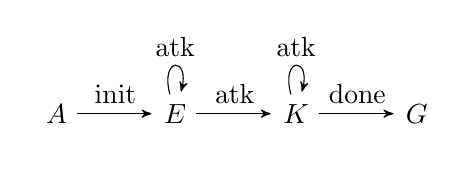
\begin{tikzpicture}
            \matrix[row sep=2cm, column sep=1cm]{
                \node (A) {$A$} ; \&
                \node (E) {$E$} ; \&
                \node (K) {$K$} ; \&
                \node (G) {$G$} ; \\
            } ;

            \graph[use existing nodes] {
                A ->[edge label={init}]
                E ->[edge label={atk},loop above]
                E ->[edge label={atk}]
                K ->[edge label={atk},loop above]
                K ->[edge label={done}] G ;
            } ;
        \end{tikzpicture}
    \end{center}
\end{frame}

\end{document}
